\documentclass{hw}

\usepackage{minted}

\begin{document}
\makeheader{1}

\begin{enumerate}
\item Dr. Martin has emailed you the data set, hmwk1.txt, which gives the time evolution of a
certain quantity of interest to him. Using R, plot the original data. In addition, using R’s ma()
function, plot a smoothed version of the data. What attribute of the original data is hidden by
referring only to the smoothed data?
\begin{quote}
\inputminted{r}{num_one.R}
The output of the above code is\\
\begin{minipage}{0.5\textwidth}
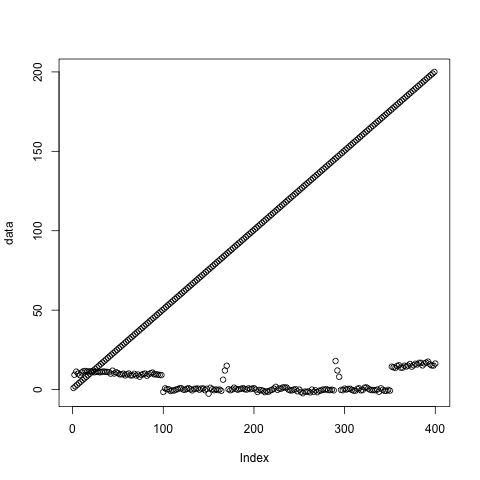
\includegraphics[scale=0.4]{01data_plot}
\end{minipage}
\begin{minipage}{0.5\textwidth}
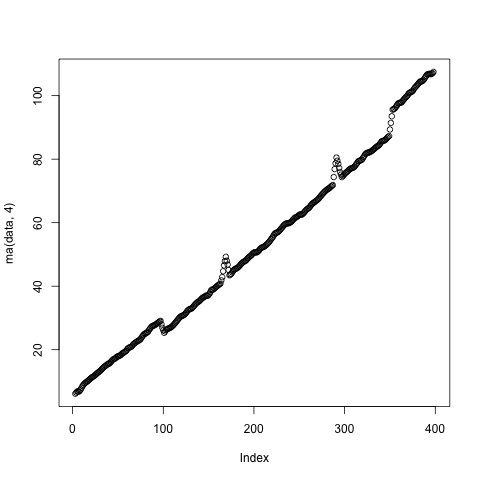
\includegraphics[scale=0.4]{01data_smoothed}
\end{minipage}
When the data is smoothed, the outlying points are lost.
\end{quote}

\newpage
\item Dr. Martin has emailed to you the data set, co2.txt. The data represents 16 years of
collecting monthly $CO_{2}$ data on the island of Hawaii, with the first year of $CO_{2}$ starting
in January of 1958. a) Using R, plot the data. b) Using R’s stl() command, plot the 1. trend, 2.
seasonal, and 3. irregular components of the data.
\begin{quote}
\inputminted{r}{num_two.R}
\begin{minipage}{0.5\textwidth}
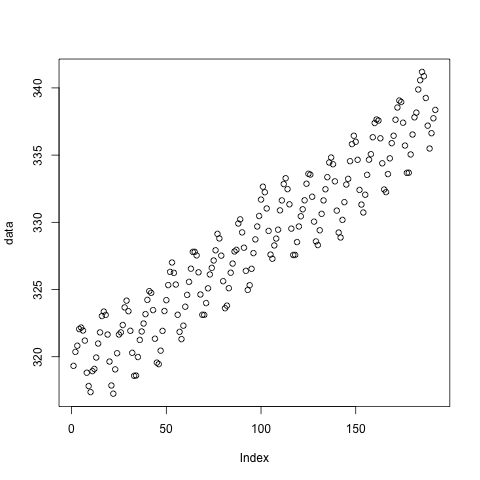
\includegraphics[scale=0.4]{02data_plot}
\end{minipage}
\begin{minipage}{0.5\textwidth}
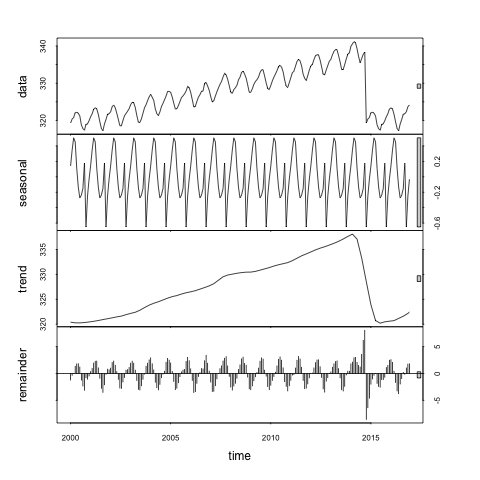
\includegraphics[scale=0.4]{02seasonal}
\end{minipage}
\end{quote}

\newpage
%% data <- Read.table('myfile.txt')
%% lm(data[,2]~data[,2]+data[,1]) will return equation of lakebed plane
%% Use Mathematica to predict where the depth is less than 5 on lakebed plane
%% The equation needs to be such that plane.z < 5
\item The following table gives the depth $Z$ of water in feet for surface points with rectangular
coordinates $X, Y$ in meters. The depth of measurements were made at low tide. Your ship has a draft of 5
feet. What region should you avoid within the rectangle $[75, 200] \times [-50, 150]$?
\begin{center}
\begin{tabular}{c | c | c}
X & Y & Z\\
\hline
129.0 & 7.5 & 4\\
140.0 & 141.5 & 8\\
108.5 & 28.0 & 6\\
88.0 & 147.0 & 8\\
185.5 & 22.5 & 6\\
195.0 & 137.5 & 8\\
105.5 & 85.5 & 8\\
157.5 & -6.5 & 9\\
107.5 & -81.0 & 9\\
77.0 & 3.0 & 8\\
162.0 & -66.5 & 9\\
162.0 & 84.0 & 4\\
117.5 & -38.5 & 9
\end{tabular}
\end{center}

\inputminted{r}{lakebedr.R}
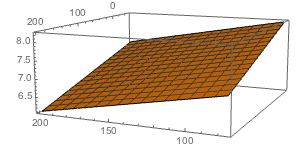
\includegraphics[scale=0.7]{three_plot}
\noindent\\
The entire area appears to be safe. However, the plane is the result of a best fit, so the corner
of the lakebed should be avoided just to be sure.

\newpage
\item My full name is James Elder Martin - numerically this corresponds to the vector 10, 1, 13, 5,
19, 5, 12, 4, 5, 18, 13, 1, 18, 20, 9, 14. Type the numerical representation of your own full name
into R as a single vector. Then issue the command, source(``batch.R"), and then (instructions for
next calling batch.R are detailed in the comments of the file, batch.R) produce a vector containing
batch averages, using a batch size, that is, a k, of 3.
\begin{quote}
\inputminted{r}{num_three.R}
\end{quote}
\end{enumerate}
\end{document}
